% Options for packages loaded elsewhere
\PassOptionsToPackage{unicode}{hyperref}
\PassOptionsToPackage{hyphens}{url}
%
\documentclass[
]{article}
\usepackage{amsmath,amssymb}
\usepackage{iftex}
\ifPDFTeX
  \usepackage[T1]{fontenc}
  \usepackage[utf8]{inputenc}
  \usepackage{textcomp} % provide euro and other symbols
\else % if luatex or xetex
  \usepackage{unicode-math} % this also loads fontspec
  \defaultfontfeatures{Scale=MatchLowercase}
  \defaultfontfeatures[\rmfamily]{Ligatures=TeX,Scale=1}
\fi
\usepackage{lmodern}
\ifPDFTeX\else
  % xetex/luatex font selection
\fi
% Use upquote if available, for straight quotes in verbatim environments
\IfFileExists{upquote.sty}{\usepackage{upquote}}{}
\IfFileExists{microtype.sty}{% use microtype if available
  \usepackage[]{microtype}
  \UseMicrotypeSet[protrusion]{basicmath} % disable protrusion for tt fonts
}{}
\makeatletter
\@ifundefined{KOMAClassName}{% if non-KOMA class
  \IfFileExists{parskip.sty}{%
    \usepackage{parskip}
  }{% else
    \setlength{\parindent}{0pt}
    \setlength{\parskip}{6pt plus 2pt minus 1pt}}
}{% if KOMA class
  \KOMAoptions{parskip=half}}
\makeatother
\usepackage{xcolor}
\usepackage[margin=1in]{geometry}
\usepackage{longtable,booktabs,array}
\usepackage{calc} % for calculating minipage widths
% Correct order of tables after \paragraph or \subparagraph
\usepackage{etoolbox}
\makeatletter
\patchcmd\longtable{\par}{\if@noskipsec\mbox{}\fi\par}{}{}
\makeatother
% Allow footnotes in longtable head/foot
\IfFileExists{footnotehyper.sty}{\usepackage{footnotehyper}}{\usepackage{footnote}}
\makesavenoteenv{longtable}
\usepackage{graphicx}
\makeatletter
\def\maxwidth{\ifdim\Gin@nat@width>\linewidth\linewidth\else\Gin@nat@width\fi}
\def\maxheight{\ifdim\Gin@nat@height>\textheight\textheight\else\Gin@nat@height\fi}
\makeatother
% Scale images if necessary, so that they will not overflow the page
% margins by default, and it is still possible to overwrite the defaults
% using explicit options in \includegraphics[width, height, ...]{}
\setkeys{Gin}{width=\maxwidth,height=\maxheight,keepaspectratio}
% Set default figure placement to htbp
\makeatletter
\def\fps@figure{htbp}
\makeatother
\setlength{\emergencystretch}{3em} % prevent overfull lines
\providecommand{\tightlist}{%
  \setlength{\itemsep}{0pt}\setlength{\parskip}{0pt}}
\setcounter{secnumdepth}{-\maxdimen} % remove section numbering
\usepackage{booktabs}
\usepackage{longtable}
\usepackage{array}
\usepackage{multirow}
\usepackage{wrapfig}
\usepackage{float}
\usepackage{colortbl}
\usepackage{pdflscape}
\usepackage{tabu}
\usepackage{threeparttable}
\usepackage{threeparttablex}
\usepackage[normalem]{ulem}
\usepackage{makecell}
\usepackage{xcolor}
\ifLuaTeX
  \usepackage{selnolig}  % disable illegal ligatures
\fi
\usepackage{bookmark}
\IfFileExists{xurl.sty}{\usepackage{xurl}}{} % add URL line breaks if available
\urlstyle{same}
\hypersetup{
  pdftitle={My Test File},
  pdfauthor={JDW},
  hidelinks,
  pdfcreator={LaTeX via pandoc}}

\title{My Test File}
\author{JDW}
\date{2024-09-18}

\begin{document}
\maketitle

\subsection{R Markdown}\label{r-markdown}

Set the working directory:

\section{1. How to emebed image into R
Markdnow}\label{how-to-emebed-image-into-r-markdnow}

This is an example of embedding images in your local folder into R
Markdown. For example, I have a illustration graph of the links between
packages ggplot2, gtable, grid, egg and gridExtra under the folder Mod7.

\begin{figure}
\centering
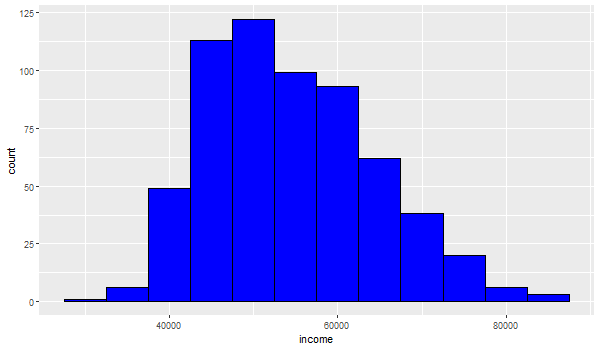
\includegraphics{Histogram_png.png}
\caption{This is my own caption}
\end{figure}

This is another way to insert the image and set the position for the
image.

\begin{figure}

{\centering 
\includegraphics[width=0.5\linewidth]{AI4} 

}

\caption{\label{fig:rein0}Resized Schematic illustration of my own file.}\label{fig:rein0}
\end{figure}

\section{2. Create a high quality figure in R
Markdown}\label{create-a-high-quality-figure-in-r-markdown}

This is an example of plotting graphs by setting the plotting area and
resolution. For example, I create a histogram below and set the width,
height and resolution in the Chunk options. You can also define the
figure size in YAML header and/or define the figure size as global chunk
option. This is my own text.

\begin{figure}[H]
  \centering
  \begin{minipage}{0.5\textwidth}
    ![\label{fig:figs1}A basic histogram of the file incomes](Test2_files/figure-latex/figs1-1.pdf) 
\end{minipage}%
  \begin{minipage}{0.5\textwidth}
    This text appears next to the image. Adjust the minipage widths as necessary.
  \end{minipage}
\end{figure}

\section{3. Refer to the figure by indexing the
figure.}\label{refer-to-the-figure-by-indexing-the-figure.}

In Figure \ref{fig:figs1}, we see that the distribution of incomes is
close to a normal distribution. In Figure \ref{fig:rein0}, we see the
illustration graph.

\section{4. Create tables using the kable function from the knitr
package.}\label{create-tables-using-the-kable-function-from-the-knitr-package.}

kable takes a data.frame as input, and outputs the table into a markdown
table, which will get rendered into the appropriate output format.

For example, let's say we wanted to share the first 6 rows of our mtcars
data.

This gives us the following output:

\begin{longtable}[]{@{}
  >{\raggedright\arraybackslash}p{(\columnwidth - 22\tabcolsep) * \real{0.2647}}
  >{\raggedleft\arraybackslash}p{(\columnwidth - 22\tabcolsep) * \real{0.0735}}
  >{\raggedleft\arraybackslash}p{(\columnwidth - 22\tabcolsep) * \real{0.0588}}
  >{\raggedleft\arraybackslash}p{(\columnwidth - 22\tabcolsep) * \real{0.0735}}
  >{\raggedleft\arraybackslash}p{(\columnwidth - 22\tabcolsep) * \real{0.0588}}
  >{\raggedleft\arraybackslash}p{(\columnwidth - 22\tabcolsep) * \real{0.0735}}
  >{\raggedleft\arraybackslash}p{(\columnwidth - 22\tabcolsep) * \real{0.0735}}
  >{\raggedleft\arraybackslash}p{(\columnwidth - 22\tabcolsep) * \real{0.0882}}
  >{\raggedleft\arraybackslash}p{(\columnwidth - 22\tabcolsep) * \real{0.0441}}
  >{\raggedleft\arraybackslash}p{(\columnwidth - 22\tabcolsep) * \real{0.0441}}
  >{\raggedleft\arraybackslash}p{(\columnwidth - 22\tabcolsep) * \real{0.0735}}
  >{\raggedleft\arraybackslash}p{(\columnwidth - 22\tabcolsep) * \real{0.0735}}@{}}
\caption{A Knitr's kable to show the first six rows of
`mtcars'}\tabularnewline
\toprule\noalign{}
\begin{minipage}[b]{\linewidth}\raggedright
\end{minipage} & \begin{minipage}[b]{\linewidth}\raggedleft
mpg
\end{minipage} & \begin{minipage}[b]{\linewidth}\raggedleft
cyl
\end{minipage} & \begin{minipage}[b]{\linewidth}\raggedleft
disp
\end{minipage} & \begin{minipage}[b]{\linewidth}\raggedleft
hp
\end{minipage} & \begin{minipage}[b]{\linewidth}\raggedleft
drat
\end{minipage} & \begin{minipage}[b]{\linewidth}\raggedleft
wt
\end{minipage} & \begin{minipage}[b]{\linewidth}\raggedleft
qsec
\end{minipage} & \begin{minipage}[b]{\linewidth}\raggedleft
vs
\end{minipage} & \begin{minipage}[b]{\linewidth}\raggedleft
am
\end{minipage} & \begin{minipage}[b]{\linewidth}\raggedleft
gear
\end{minipage} & \begin{minipage}[b]{\linewidth}\raggedleft
carb
\end{minipage} \\
\midrule\noalign{}
\endfirsthead
\toprule\noalign{}
\begin{minipage}[b]{\linewidth}\raggedright
\end{minipage} & \begin{minipage}[b]{\linewidth}\raggedleft
mpg
\end{minipage} & \begin{minipage}[b]{\linewidth}\raggedleft
cyl
\end{minipage} & \begin{minipage}[b]{\linewidth}\raggedleft
disp
\end{minipage} & \begin{minipage}[b]{\linewidth}\raggedleft
hp
\end{minipage} & \begin{minipage}[b]{\linewidth}\raggedleft
drat
\end{minipage} & \begin{minipage}[b]{\linewidth}\raggedleft
wt
\end{minipage} & \begin{minipage}[b]{\linewidth}\raggedleft
qsec
\end{minipage} & \begin{minipage}[b]{\linewidth}\raggedleft
vs
\end{minipage} & \begin{minipage}[b]{\linewidth}\raggedleft
am
\end{minipage} & \begin{minipage}[b]{\linewidth}\raggedleft
gear
\end{minipage} & \begin{minipage}[b]{\linewidth}\raggedleft
carb
\end{minipage} \\
\midrule\noalign{}
\endhead
\bottomrule\noalign{}
\endlastfoot
Mazda RX4 & 21.0 & 6 & 160 & 110 & 3.90 & 2.62 & 16.46 & 0 & 1 & 4 &
4 \\
Mazda RX4 Wag & 21.0 & 6 & 160 & 110 & 3.90 & 2.88 & 17.02 & 0 & 1 & 4 &
4 \\
Datsun 710 & 22.8 & 4 & 108 & 93 & 3.85 & 2.32 & 18.61 & 1 & 1 & 4 &
1 \\
Hornet 4 Drive & 21.4 & 6 & 258 & 110 & 3.08 & 3.21 & 19.44 & 1 & 0 & 3
& 1 \\
Hornet Sportabout & 18.7 & 8 & 360 & 175 & 3.15 & 3.44 & 17.02 & 0 & 0 &
3 & 2 \\
Valiant & 18.1 & 6 & 225 & 105 & 2.76 & 3.46 & 20.22 & 1 & 0 & 3 & 1 \\
\end{longtable}

\section{5. Refer to the tables}\label{refer-to-the-tables}

For example, let's say we wanted to share the first 10 rows of our
mtcars data.

This gives us the following output:

\begin{longtable}[t]{lrrrrrrrrrrr}
\caption{\label{tab:tabl1}A Knitr's kable to show the first ten rows of 'mtcars'}\\
\toprule
 & mpg & cyl & disp & hp & drat & wt & qsec & vs & am & gear & carb\\
\midrule
Mazda RX4 & 21.0 & 6 & 160.0 & 110 & 3.90 & 2.62 & 16.46 & 0 & 1 & 4 & 4\\
Mazda RX4 Wag & 21.0 & 6 & 160.0 & 110 & 3.90 & 2.88 & 17.02 & 0 & 1 & 4 & 4\\
Datsun 710 & 22.8 & 4 & 108.0 & 93 & 3.85 & 2.32 & 18.61 & 1 & 1 & 4 & 1\\
Hornet 4 Drive & 21.4 & 6 & 258.0 & 110 & 3.08 & 3.21 & 19.44 & 1 & 0 & 3 & 1\\
Hornet Sportabout & 18.7 & 8 & 360.0 & 175 & 3.15 & 3.44 & 17.02 & 0 & 0 & 3 & 2\\
\addlinespace
Valiant & 18.1 & 6 & 225.0 & 105 & 2.76 & 3.46 & 20.22 & 1 & 0 & 3 & 1\\
Duster 360 & 14.3 & 8 & 360.0 & 245 & 3.21 & 3.57 & 15.84 & 0 & 0 & 3 & 4\\
Merc 240D & 24.4 & 4 & 146.7 & 62 & 3.69 & 3.19 & 20.00 & 1 & 0 & 4 & 2\\
Merc 230 & 22.8 & 4 & 140.8 & 95 & 3.92 & 3.15 & 22.90 & 1 & 0 & 4 & 2\\
Merc 280 & 19.2 & 6 & 167.6 & 123 & 3.92 & 3.44 & 18.30 & 1 & 0 & 4 & 4\\
\bottomrule
\end{longtable}

In Table \ref{tab:tbl1}, we see the first \textbf{10} rows of the
dataset ``mtcars''.

\end{document}
